\section{Process} \label{sec:process}


Throughout the Rubin pre-operations and operations phases, annually in May each team will look back at what was planned, what was achieved, do a full review of its activities, and propose a high level plan for the following (US fiscal) year.
This is standard practice in other high energy physics experiments as well, the scrub allows the facility to continuously evolve its operating plan, taking critical input from the people that understand best what is really needed, in Rubin’s case that is the Team Leaders.
Following the National Science Foundation and Department of Energy joint annual review of Rubin Operations the Rubin Operations Directors office together with department heads sets the major milestones for the next US fiscal year (FY) starting 1st October. This includes looking at the status of major milestones for the current year and ascertaining whether any of those need to carry over into the next FY.
With the major milestones set, the Director’s office kicks off the month long annual scrub process, see \autoref{fig:timeline} in which the department heads start down stream planning with their teams. This is the “homework” phase of the scrub where teams are looking at:

\begin{itemize}
\item status of minor milestones for the current FY
\item setting minor milestones that would contribute to accomplishing the new major milestones for the next FY
\item based on activities needed to achieve the minor milestones and risk mitigation plans the teams review planned resources both labor and non-labor
\item if there is a mismatch between resources needed and the resources available the team will propose changes during this scrub period through the tool (described in the next section).

\end{itemize}


\begin{figure}[hb!]
\begin{centering}
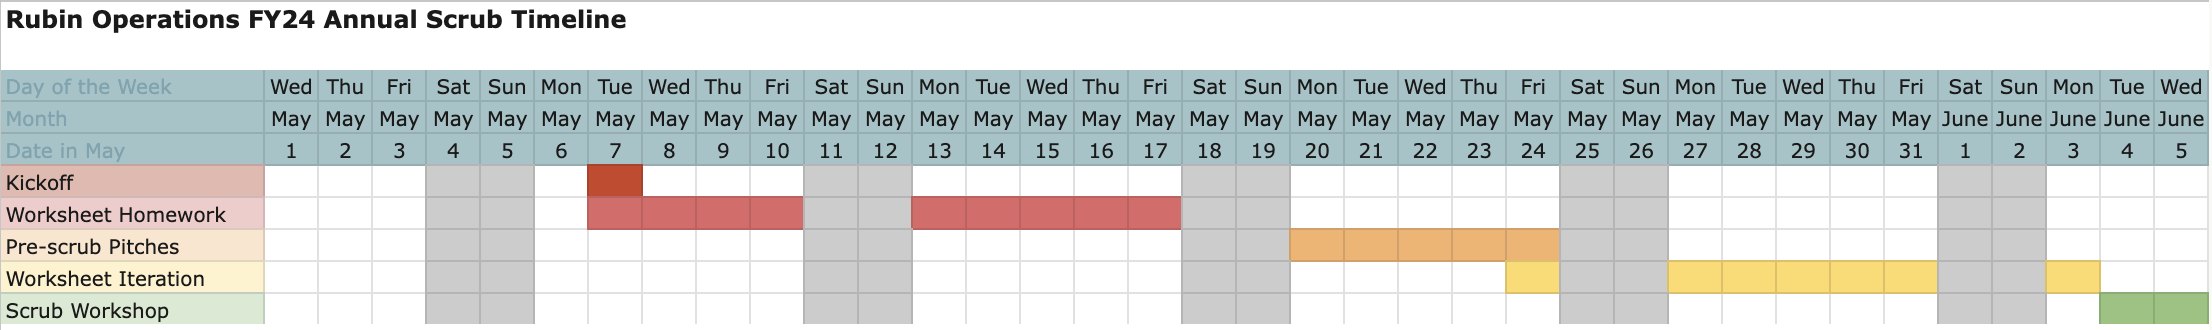
\includegraphics[width=1.0\textwidth]{Figure1Scrubtimeline}
	\caption{Scrub timeline
\label{fig:timeline}}
\end{centering}
\end{figure}
Having completed the above homework, in the tool provided, the scrub moves into the “pitches” phase. Department heads and team leads prepare short presentations, for which a template is provided, to pitch the needed changes to the Director’s office. As additional resource requests from one department could impact another, all department leads and team leads are invited and encouraged to attend all pitches. Currently in Rubin the 15-30 minutes team level pitches are carried out per department in virtual format. This is in contrast to the ATLAS Experiment where the teams come together for an in-person gathering to present pitches.

After the pitches phase is complete a period of iteration takes place between the director’s office and department/team to reach an agreement on the changes.

The directors office is aggregating the labor and non-labor baseline vs proposed changes across the Rubin departments to ensure the program remains overall within the defined financial envelope. This is one of the reasons for the back and forth iterations and negotiations as priorities have to drive this process.

After agreement the changes are implemented by propagating them throughout the Rubin planning tools culminating in the spending plan for the next FY and definition of Statements of Work for the contracts enabling requisitions to be input in time for contracts to be placed.

With the resources now updated across all the tools teams can start realistically planning for the coming FY by defining the tasks and activities that will lead to completion of the defined minor milestones within the boundaries of the available resources. Work then commences at the start of the FY. The activity planning is done in an Atlassian tool called Jira where the milestones are defined enabling downstream and upstream traceability between milestones to tasks.The Jira tool is outside the scope of this paper.

From the start of the FY the Director’s office takes inputs, such as overhead rates, escalation rates etc, as defined by the managing organization and preps the tools for the next annual scrub and so the cycle continues, see see \autoref{fig:cycle}.


\begin{figure}
\begin{centering}
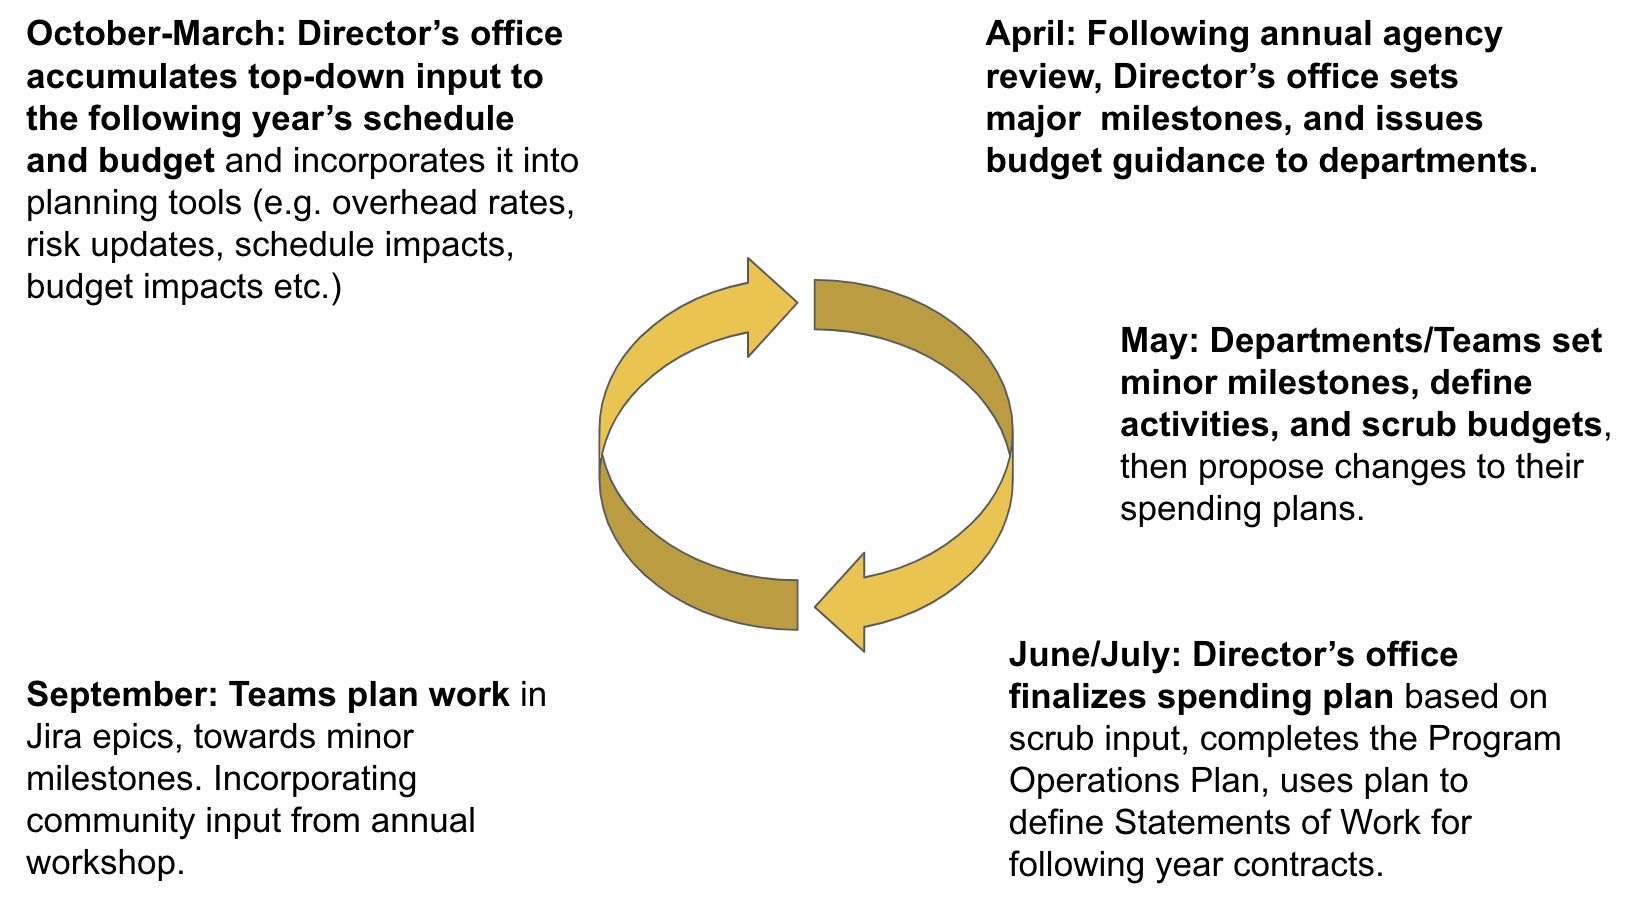
\includegraphics[width=1.0\textwidth]{Figure2AnnualPlanningScrubCycle}
	\caption{The annual planning and scrub cycle
\label{fig:cycle}}
\end{centering}
\end{figure}
